\section{Evaluation}
In this section, we use a series of experiments to show that
given an interested SDN (sub)network with rules $SN(R)$, our approach can 
(1) transform $SN(R)$ to a single OpenFlow switch without any loss of forwarding logic in network $SN(R)$;
(2) save emulation resources such as number of total rules in the network and emulation runtime.

We consider a tree-topology network with two topological parameters: depth $d$ and fanout $f$.
Such a tree network $tree(d, f)$ can connect $f^d$ hosts with $\frac{f^d - 1}{f-1}$ switches in total.
Though not known as a scalable network architecture
(a good scalable alternative will be fat-tree topology),
it is good for demonstration purpose since the tree topology is well-structured and
all hosts in it are potentially fully-connected with at most $2d$ hops.

\subsection{Preserve Forwarding Logic}
In the following set of experiment, we demonstrate that forwarding logic in $SN(R)$ are
perfectly preserved by the big-virtual-switch approach.
We generate forwarding logic in tree-topology network by create paths between random host pairs.
One can find the shortest path between a pair of hosts $(s, d)$ with
a layer-two learning switch controller application.
Traversing the tree up and down in breadth-first-search style, learning switch application
can automatically install OpenFlow rules on each hop once we initiate \texttt{ping} between
the given pair of host.
More specifically, we start a tree-topology network $net_1$ in Mininet\cite{Mininet},
connecting all switches to a l2\_learning switch controller\cite{Pox}.
For any network host $s$, we randomly generate a list of distinct hosts $dsts$,
and let $s$ \texttt{ping} each host $dst \in dsts$.
After doing this \texttt{ping} process for all hosts, necessary rules will be available on
certain switches.
We then take a snapshot of this network by
\begin{enumerate}
\item Recording the network topology, e.g. host to switch and switch to switch connections.
\item Logging all rules on all switches with \texttt{ovs-ofctl dump-flows} commands
\end{enumerate}
We then feed the above information as input in order to generate the rules of the new big switch
and port mappings according to procedures and algorithms presented in section~\ref{Sec:Design}.
Now we create another emulated network with one switches and
the same number of hosts as $net_1$ using Mininet.
This big-switch network $net_2$ has one OpenFlow switch $bs$ that connects to $f^d$ hosts using
appropriate port numbers deducted from both the $PortMap$(from Algorithm~\ref{Alg:GenAllRules})
and link information(from $net_1$'s topology record).
Besides, rules generated by Algorithm~\ref{Alg:GenAllRules} are manually(instead by controller)
installed on $bs$ by \texttt{ovs-ofctl add-flow} commands.

To proof that our approach can preserve the existing forwarding logic in original network,
we generate a matrix $\mathcal{M}$ of size $f^d$ by $f^d$, each element randomly picked
from the integer range [1, 10].
In both emulated network $net_1$ and $net_2$, host $i$ will send $\mathcal{M}[i][j]$
packets to host $j$ using \texttt{ping}, if $i \neq j$.
To prevent l2\_learning switch controller from installing new rules in $net_1$, we take down
the pox controller in this stage.
The result of this experiment is a matrix $\mathcal{R}_k$ where $\mathcal{R}[i][j]$ denote
the number of successfully received \texttt{ping} packets by host $i$ from host $j$ in $net_k$.

We have repeated this experiment for different ($d, f$) pairs $\in$
\{(2, 3), (2, 4), (3, 3), (3, 4), (4, 3), (4, 4)\} and found that
$\mathcal{R}_1 = \mathcal{R}_2$ holds in all six experiment settings.
As an example, we have visualized $\mathcal{R}_1$ and $\mathcal{R}_2$ for ($d=2, f=3$) as gray image
in Figure~\ref{Fig:PingMatrix1} and Figure~\ref{Fig:PingMatrix2},
where brightness is proportional to number of received packets.
In this way it is easy to see that $\mathcal{R}_1$ and $\mathcal{R}_2$ are identical.

\begin{figure*}[t]
        \centering
        \subfloat[Packets received in $net_1$] {
                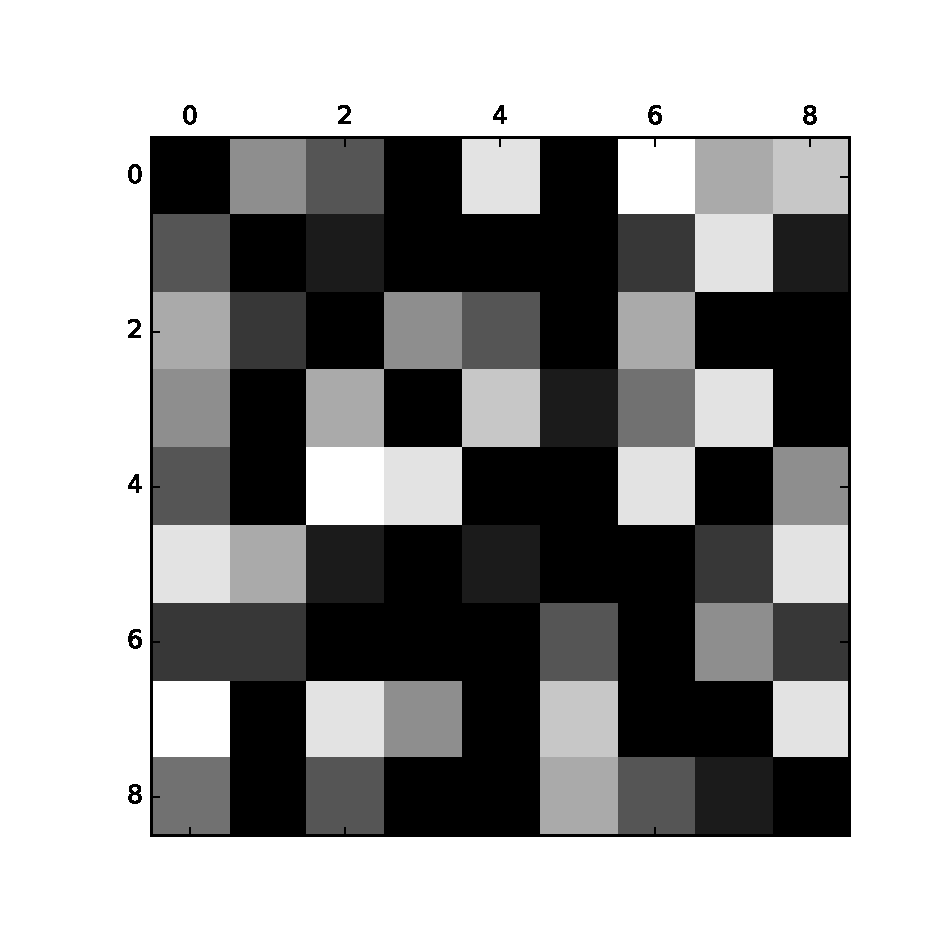
\includegraphics[scale=.5]{figures/ping_mat_2_3.eps}
                \label{Fig:PingMatrix1}
        }
        \subfloat[Packets received in $net_2$] {
                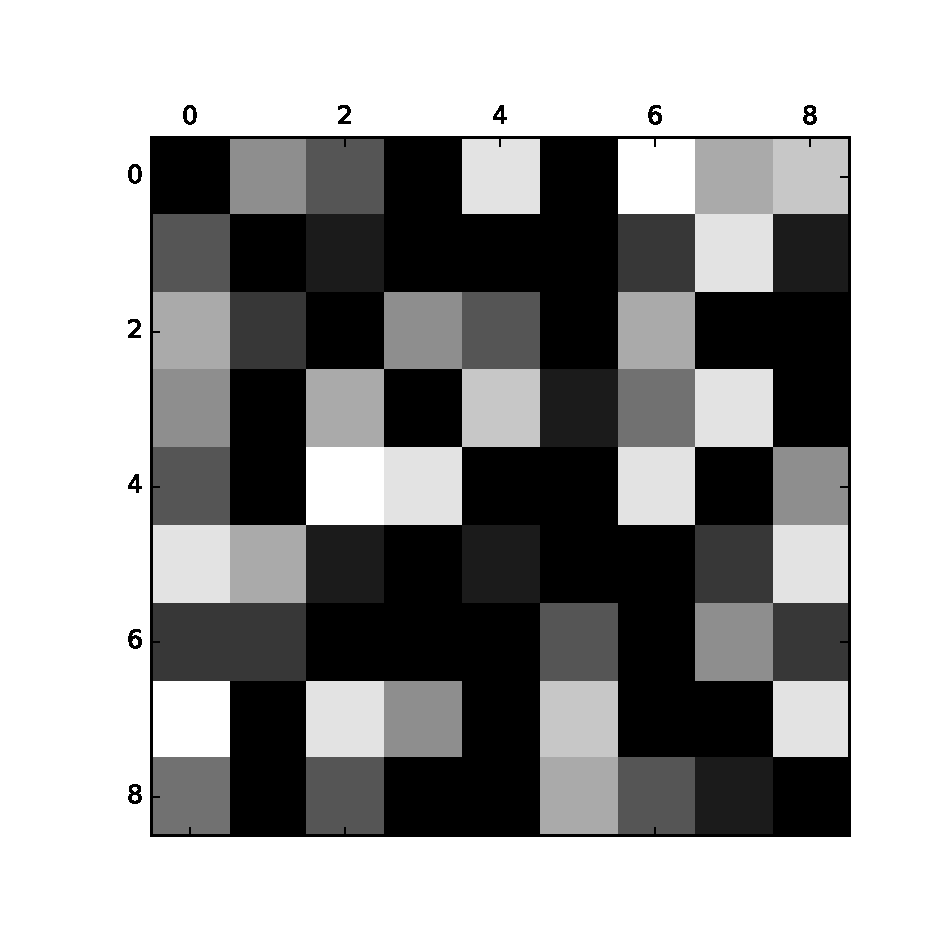
\includegraphics[scale=.5]{figures/bs_ping_mat_2_3.eps}
                \label{Fig:PingMatrix2}
        }
        \caption{$\mathcal{R}_1$ and $\mathcal{R}_2$ of two emulated networks ($f=3, d=2$)}
        \label{Fig:TwoPingMatrix}
\end{figure*}

